\chapter{Implement\'aci\'o}\label{chapter:implementation}
Ebben a fejezetben a "WatchWithFriends" alkalmazás implementációs folyamatát mutatom be.
\section{Szerver oldali logika}
\subsection{Entity Framework és Data projekt}
Az adatintegritás és az adatmanipuláció kezelésének centralizálása érdekében létrehoztam egy különálló projektcsoportot, amely specifikusan az adatkezelési logika implementációjáért felel. Ebben a dedikált modulban helyeztem el az adatbázis tábláinak sémáját, valamint az adathozzáférési réteget képviselő repository-kat.
\\
A modul architektúrája rugalmas és jól skálázható módon épül fel, köszönhetően az Entity Framework integrációjának. Az Entity Framework ORM (Object-Relational Mapping) képességeit kihasználva, egyszerűsítem és automatizálom az adatbázis műveleteket, csökkentve ezzel az ismétlődő kód és az esetleges hibák számát.
\\
A modell definíciók és az adatbázis kontextus is ebbe a projektcsoportba kerültek, így biztosítva, hogy az adatmodellek és az adatbázis-sémák közötti szoros kapcsolat koherens és könnyen kezelhető maradjon. Az egész rendszer így válik áttekinthetővé és könnyen karbantarthatóvá.
\\
Ezen architektúra alkalmazásával nem csak az adatkezelés egyszerűsödik, de a jövőbeli fejlesztések és bővítések is gördülékenyebben, valamint hatékonyabban valósíthatók meg.
\subsubsection{Modellek}
A modellek az adatbázisban lévő táblákat reprezentálják, és a kontextus segítségével tudom őket kezelni.

A táblákat reprezentáló modelleknek minden tulajdonsága egy oszlop az adatbázisban.
A modellekben találhatóak navigációs tulajdonságok is, amelyek segítségével a modellek közötti kapcsolatokat tudom megvalósítani.
A táblákat a migrációk segítségével tudom létrehozni, amelyek a modellek alapján generálódnak, majd az update-database parancs kiadásával tudom őket alkalmazni az adatbázison.

\subsubsection{Kontextusok}
A komplex adatkezelési igényeket kielégítendő, a szoftverarchitektúrámban két különálló adatbázis-kontextust implementáltam. Az első, a "WatchWithFriendsDBContext", főként a felhasználói információkat és a képmegosztás funkciókat kezeli. Ennek az adatállománynak az SQL Server adatbázisban való tárolása biztosítja az adatintegritást és a tranzakcionális biztonságot.

A másik kontextus, a "RoomsDBContext", azonban egészen más jellegű adatokat adminisztrál: itt a szobák és a videók információit kezelem. Erre az adatrétegre egy InMemory adatbázist alkalmazok. Ezzel a megoldással két fontos célt érek el. Egyrészt, az InMemory adatbázis lehetővé teszi a gyors és rugalmas adatmanipulációt, optimális azokhoz a szobákhoz és videókhoz, amelyek volatilis jelleggel bírnak és nem szükségesek hosszútávú tárolásra. Másrészt, a szerver leállításával automatikusan törlődnek ezek az adatok, így nincs szükség manuális karbantartásra ezen a fronton.

A két különböző kontextus párhuzamos működése lehetővé teszi az adatrétegek elkülönítését és a szoftver komponenseinek független skálázhatóságát, miközben az adatintegritás és a rendelkezésre állás is megmarad.
\subsubsection{Repository réteg}
A repository-k segítségével tudom kezelni az adatbázist, és a modelleket.
Fontosnak tartottam az async műveletek használatát, mert így a szerver nem blokkolódik, és a kliensek is gyorsabban kapják meg a válaszokat.
\subsubsection{Extension metódus}
A kiterjesztési metódus, amely lehetővé teszi a repository-k és a service-k regisztrálását a DI konténerben, valamint a kontextusok létrehozását, és más fejlesztési eszközök alkalmazását, például Swagger és CorsPolicy.
\vspace{1em}
\subsection{Szerver oldali logika és végpontok}
A szerver oldali logika az alkalmazás "háttere", itt történik minden, ami az adatok manipulációjával, az üzleti szabályok végrehajtásával és az erőforrások menedzsmentjével kapcsolatos. A végpontok (endpoints) a szerver oldali logika speciális részei, amelyek meghatározzák, hogy a kliens hogyan interakciózik a szerverrel.
\subsubsection{Service réteg}
A service réteg az alkalmazás üzleti logikáját tartalmazza általában. Ide tartoznak azok a függvények és metódusok, amelyek nem közvetlenül az adatok eléréséhez vagy a felhasználói felülethez kapcsolódnak, hanem inkább az alkalmazás "logikáját" képezik. Például ide sorolható a felhasználók hitelesítése bejelentkezéskor, a felhasználók regisztrálása, valamint egyes szobákhoz kapcsolódó műveletek.

A service rétegben található szolgáltatások, más néven szolgáltatásos osztályok, az alkalmazás különböző üzleti funkcióit valósítják meg. Az elvárás az, hogy ezek a szolgáltatások jól elkülönüljenek egymástól, azaz minden egyes service specifikus üzleti logikát kezeljen, és ne fedjen át más szolgáltatások feladatait. Ennek eredményeként az egyes szolgáltatások tiszták, jól definiáltak, és egységesen kezelik az adott üzleti funkciót.

\subsubsection{Controller réteg}
A controller réteg felelős a végpontok kezeléséért az alkalmazásban. Ezek a végpontok az alapját képezik a kliens és a szerver közötti kommunikációnak. A végpontok meghatározzák, hogy hogyan interakciózik a kliens a szerverrel. Ők fogadják a kliens kéréseit és generálnak válaszokat rájuk.
A végpontok azok a konkrét helyek az alkalmazásban, ahol a kliens eléri a szervert. Tehát minden kliens által kiváltott műveletet megvalósító végpont a controller rétegbe kerül. Itt történik meg a kliens kérésének kezelése, az üzleti logika meghívása, az adatok feldolgozása és a válasz előkészítése a kliens számára.
Az egyes végpontokhoz tartozó logika elérése érdekében a szükséges szolgáltatások, vagyis a servicek, azok a végpontokba vannak injektálva. Ez lehetővé teszi a controller réteg számára, hogy elérje az üzleti logikát és adatelérést biztosító szolgáltatásokat, amelyekre szüksége van a kliens kéréseinek megfelelő kezeléséhez és a válaszok generálásához.
\subsubsection{Hub réteg}
Az implementáció lényege, hogy a hubok hívásait a controllerek végzik, viszont ezek a hubok egy teljesen másik rétegben helyezkednek el. Amikor a különböző endpointokat hívják, a hub osztja szét a válaszokat azoknak a felhasználóknak, akik fel vannak iratkozva a hubra. Ezzel a megközelítéssel a válaszok célzottan és hatékonyan jutnak el az érintett felhasználókhoz, még akkor is, ha a hub és a controllerek különböző rétegekben találhatók. Ez lehetővé teszi a jobb szervezettséget és a könnyebb karbantarthatóságot az alkalmazás különböző részein.

\begin{figure}[H]
    \centering
    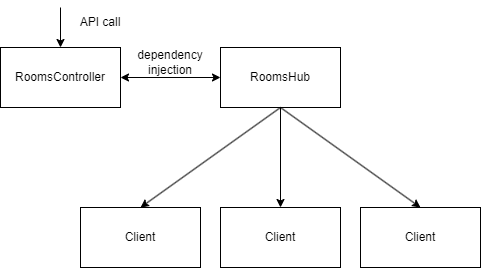
\includegraphics[width=14.0truecm]{images/roomshub.png}
    \caption{RoomHub működésének folyamata}
    \label{fig:frontend_architecture}
\end{figure}

\section{Kliens oldali logika}
\subsection{React projekt}
A kliens oldali logika a felhasználói felületet és a felhasználói interakciókat kezeli az alkalmazásban. Gyakran előfordul, hogy a kliens oldali kód aszinkron módon kommunikál a szerverrel, hogy adatokat kérjen vagy küldjön.

Az adatok küldésére és fogadására API hívásokat használok a React alkalmazásban. Ezeket az API hívásokat a axios \cite[]{axios} nevű HTTP kliens könyvtárral valósítottam meg. Az axios lehetővé teszi a kérések küldését a szervernek és a válaszok fogadását.

Az axios beállításait külön fájlban tárolom, így könnyen módosíthatóak és karbantarthatóak maradnak. Ez segít abban, hogy az alkalmazás konfigurációját könnyedén kezelni lehessen, és az egyszerűsítse a fejlesztési folyamatot.

Az egyes axios végpontokat egy OpenAPI generátorral generáltattam, amely a szerver által előállított swagger.json fájlból generálta a végpontokhoz szükséges definíciókat. Ez a megközelítés segíti a konzisztens és pontos végpontkezelést, valamint minimalizálja az emberi hibák lehetőségét a kézi végpontdefiníciók létrehozásával szemben.

\subsection{Környezeti változók}
Az env változók validására a joi \cite[]{joi} nevű könyvtárat használom, amely segítségével tudom a változókat ellenőrizni, hogy megfelelnek-e a várt típusnak, illetve, hogy megvannak-e adva.

\subsection{Router}
A Router egy olyan elem vagy komponens, amely lehetővé teszi a különböző oldalak megjelenítését az alkalmazásban, és irányítja a navigációt a felhasználók számára.

A példa bemutatja a React alkalmazásban használt Router használatát. A fő elemek a következők:
\begin{lstlisting}[style=Csharp,caption={Router}]
<BrowserRouter>
    <Navbar />
    <CommonSrtyles.PageContainer>
      <Routes>
        <Route path="/" element={<HomePage />} />
        <Route path="/rooms" element={<RoomsPage />} />
        <Route path="/profile" element={<ProfilePage />} />
        <Route path="/friends" element={<FriendsPage />} />
        <Route path="/room/:id" element={<RoomPageWithProvider />} />
      </Routes>
    </CommonSrtyles.PageContainer>
</BrowserRouter>
\end{lstlisting}
\vspace{1em}
\begin{itemize}
\item \texttt{BrowserRouter} komponens: Ez a Router fő komponense, amely kezeli az URL változásait és irányítja a routingot az alkalmazásban.
\item \texttt{Navbar} komponens: Ez a navigációs sáv, amely segíti a felhasználókat az alkalmazás különböző részei közötti váltásban.

\item \texttt{CommonStyles.PageContainer} komponens: Ez a tartalom közös stílusokat tartalmazó konténer komponense, ami egységes megjelenítést biztosít az alkalmazás különböző részeinek.

\item \texttt{Routes} komponens: Ez a Router része, amely tartalmazza az alkalmazás útvonalait és az ezekhez tartozó megjelenítendő komponenseket.

\item \texttt{Route} komponensek: Ezek a Route komponensek definiálják az útvonalakat és az ezekhez tartozó megjelenítendő komponenseket.
\end{itemize}
\vspace{1em}

\subsection{Komponensek}
A React komponensek a UI logikájának egységei, és lehetnek függvény vagy osztály alapúak. Függvényes komponensek egyszerűbbek és könnyebben kezelhetőek, míg az osztály alapúak sokkal több beépített metódust és ciklusfüggvényt kínálnak.
A komponenseknek tulajdonságai (props) amivel a komponensek közötti adatáramlást valósítottam meg.
A komponenseket alkomponensekre bontottam, hogy a kód minél jobban átlátható legyen, és a komponensek újra felhasználhatóak legyenek.
Ezt a  styled-components \cite[]{styled-components} könyvtár segítségével készítettem, amely lehetővé teszi a CSS kódok beágyazását a komponensekbe.
Így egyszerűen adom meg a komponensek stílusát, és a komponensek újra felhasználhatóak lettek.
Illetve ezekből a komponensekből összeállt egy nagyobb komponens.
\vspace{1em}
\subsection{Context API}
Az alkalmazásban felhasznált közös adatokat, mint például a felhasználói adatok és a szobákkal kapcsolatos információk, a Context API segítségével valósítottad meg.

A Context API egy olyan eszköz a React-ben, amely lehetővé teszi a komponensek közötti adatmegosztást anélkül, hogy mély komponensfa-navigációt kellene alkalmazni. A Context API létrehoz egy globális állapotot, amely elérhetővé válik a komponensek számára, amelyek szükségét érzik az adatoknak.

Ez a megközelítés különösen hasznos olyan adatok esetén, amelyeket több különböző komponens is használ, mivel megakadályozza a prop drillinget és egyszerűsíti az adatok kezelését.

A felhasználói adatok és a szobákkal kapcsolatos információk esetén a Context API segítségével létrehoztál két külön állapotkezelő kontextust, amelyek tárolják ezeket az adatokat. Ezáltal bármely olyan komponens, amelynek szüksége van ezekre az adatokra, egyszerűen hozzáférhet hozzájuk a megfelelő kontextus felhasználásával, anélkül, hogy közvetlenül propokat kellene átadni.
\\
\begin{lstlisting}[style=Csharp,caption={Context API}]
import { createContext, useState } from "react";

//Context API inicializalasa

interface AuthContextType {
    //valtozok es metodusok
}

export const AuthContext =
    createContext<AuthContextType | null>(null);

//Context API Provider

export const AuthProvider = ({ children }:
 { children: React.ReactNode }) => {
    //adat es setter
    return (
        <AuthContext.Provider
            value={{
                //adat es setter
            }}
        >
            {children}
        </AuthContext.Provider>
    );
};

//Context API hasznalata
const authContext = useContext(AuthContext);
\end{lstlisting}
\vspace{1em}
\subsection*{Videók adatainak lekérdezése}
Az alkalmazásban a videók adatainak lekérdezéséhez a YouTube Data API-t használtam. Ehhez először generálnom kellett egy hozzáférési tokent, amely segítségével hozzáfértem a YouTube ingyenes API szolgáltatásához. Az API segítségével lekérdezhettem a videókhoz tartozó thumbnail linkjét, címüket és leírásukat is, bár végül csak a thumbnail-eket és a címeket használtam fel a továbbiakban.

\begin{lstlisting}[style=Csharp,caption={Youtube Data API használata}]
const getYoutubeVideoIdFromUrl = (url:string) => {
    const regExp 
        = /^.*(youtu\.be\/|v\/|e\/|u\/\w+\/|embed\/|v=)([^#&?]*).*/;
    const match = url.match(regExp);
    return match && match[2].length === 11 ? match[2] : null;
};

export const getVideoDetails = async (videoUrl:string) => {
    const videoId = getYoutubeVideoIdFromUrl(videoUrl);
    if (!videoId) {
        throw new Error('Invalid YouTube video URL.');
    }

    const API_ENDPOINT 
        = `https://www.googleapis.com/youtube/
        v3/videos?id=${videoId}&key=${YOUTUBE_API_KEY}&part=snippet`;

    try {
        const response = await fetch(API_ENDPOINT);
        const data = await response.json();

        if (data.items.length > 0) {
            return data.items[0].snippet;
        } else {
            throw new Error('YouTube video title not found.');
        }
    } catch (error) {
        throw new Error('Error fetching YouTube video title: '
            + error);
    }
};
\end{lstlisting}
\vspace{1em}
\begin{itemize}
\item \textbf{getYoutubeVideoIdFromUrl} fügvény lehetővé teszi, hogy kinyerjük a YouTube videók egyedi azonosítóját az URL-ekből. Az URL-nek bizonyos előírt mintának kell megfelelnie, hogy ez a függvény megfelelően működjön. Ezt az előírt mintát egy bonyolult reguláris kifejezés segítségével ellenőrizzük, amely összehasonlítja az URL-t a YouTube videók URL-jének ismert mintájával.

Ez a függvény egyfajta szűrőként működik: ha az URL megfelel az elvárt mintának, akkor a függvény visszaadja az azonosítót. Ellenkező esetben pedig jelzi, hogy az adott URL nem felel meg a YouTube videók URL-sémájának.

\item \textbf{getVideoDetails} funkció azért jött létre, hogy lehetővé tegye számunkra a YouTube videók részletes adatainak lekérését. Ennek eléréséhez az API hívás URL-jébe (API\_ENDPOINT) beillesztjük azt az azonosítót, amit a getYoutubeVideoIdFromUrl metódusból nyerünk ki, valamint a saját generált hozzáférési kulcsunkat.

\end{itemize}

\section{Videók lejátszása kliens oldalon}
A videók lejátszásához ReactPlayert használok, amely egy univerzális videó lejátszó komponens a React alkalmazások számára. Ez a könyvtár támogatja a legnépszerűbb videómegosztó platformokat, mint a YouTube, Vimeo és sok más mellett közvetlen videófájl formátumokat is. A ReactPlayer egyszerűsége és rugalmassága lehetővé teszi számomra, hogy könnyedén integráljam a videókat a webes projektjeimbe, testreszabott vezérlőkkel és beállításokkal, mint például az automatikus lejátszás, hangerőszabályozás, ismétlés és kezdőidőpont megadása.

Ez a komponens különösen hasznos a felhasználói élmény szempontjából, mivel adaptív, így a videók tökéletesen megjelennek minden eszközön és képernyőméreten. A ReactPlayer API-jának köszönhetően teljes körű kontrollt kapok a videó lejátszás felett, beleértve az állapotváltozások kezelését, hibakezelést és programozott vezérlést is, ami nagyban hozzájárul az alkalmazásom funkcionalitásának és interaktivitásának bővítéséhez.
\\
\textbf{Főbb metódusai}
\begin{itemize}
\item \texttt{play():} Ez a metódus elindítja a videó lejátszását.
\item \texttt{pause():} A videó lejátszásának szüneteltetésére szolgál.
\item \texttt{stop():} Megállítja a videót, és visszaállítja a lejátszási pozíciót a kezdeti állapotba.
\item \texttt{seekTo(fraction, type):}
A videó adott részére ugrik. Az fraction egy szám, amely a videó hosszának egy adott százalékát jelenti (ha a type 'fraction'), vagy másodpercben megadott időpont (ha a type 'seconds').
\item \texttt{getDuration():} Visszaadja a videó teljes hosszát másodpercben.
\item \texttt{getCurrentTime():} Lekéri a jelenlegi lejátszási pozíciót másodpercben.
\item \texttt{getInternalPlayer(key):}
Lehetővé teszi a belső lejátszó objektum elérését, amely specifikus funkciók eléréséhez lehet hasznos, például ha közvetlenül hozzá szeretnénk férni a YouTube API-hoz.
\end{itemize}
\textbf{Főbb esemény kezelői}
\begin{itemize}
  \item \texttt{onReady}: Akkor hívódik meg, amikor a lejátszó teljesen betöltődött és kész a lejátszásra. Ez tökéletes időpont például egy lejátszás gomb aktiválására.
  \item \texttt{onPlay}: Ez az eseménykezelő akkor fut le, amikor a videó lejátszása elkezdődik. Használható a lejátszás állapotának nyomon követésére.
  \item \texttt{onPause}: Akkor aktiválódik, amikor a videó lejátszását szüneteltetik. Segítségével reagálhatunk a lejátszás szüneteltetésére.
  \item \texttt{onStop}: Ezt az eseménykezelőt akkor hívja meg a rendszer, amikor a videó lejátszása megáll.
  \item \texttt{onBuffer}: Ez az esemény akkor történik, amikor a videó buffereződik. Hasznos lehet a felhasználói felületen egy töltési állapot megjelenítéséhez.
  \item \texttt{onEnded}: Akkor hívódik meg, amikor a videó végére ér és leáll a lejátszás. Ez lehetőséget ad arra, hogy reagáljunk a videó befejezésére, például másik videó automatikus indításával.
  \item \texttt{onError}: Ez az eseménykezelő akkor fut le, ha a videó lejátszása során hiba történik. Információt nyújthat a hiba természetéről, lehetővé téve a hibakezelési logika implementálását.
  \item \texttt{onDuration}: A videó teljes időtartamának információját adja meg, amikor ez elérhetővé válik. Ez segíthet a lejátszási csúszka vagy időjelző frissítésében.
  \item \texttt{onSeek}: Amikor a felhasználó keres a videón belül, ez az eseménykezelő reagál a keresési műveletre, lehetővé téve, hogy nyomon követhessük a lejátszási pozíció változását.
\end{itemize}
\vspace{0em}
\textbf{Kapcsolat létesítése a RoomHub-al}
\\
Először is, az eseményekre való feliratkozáshoz szükségem volt a kapcsolat létrehozására a hubot üzemeltető szerverrel. Ezt a SignalR könyvtár HubConnectionBuilder metódusának segítségével értem el. Ezt követően regisztráltam a szobákhoz kapcsolódó események figyelésére. A feliratkozás sikeres befejeztével meghívódott a JoinRoom API metódus, amely segítségével a klienst hozzárendeltem a megfelelő szobához.
\begin{lstlisting}[style=Csharp,caption={Kapcsolat létrehozása a szerverrel és csatlakozás a szobához}]
const startConnection = async () => {
    try {
        const roomConnection = new signalR.HubConnectionBuilder()
            .withUrl(AppConfig.getConfig().apiUrl + 'roomHub')
            .withAutomaticReconnect()
            .build();

        subscribeHubEvents(roomConnection);
        await roomConnection.start();
        if(!authContext?.currentUser)
        {
            throw new Error('User not authenticated');
        }
        if(roomConnection.connectionId === null 
        || roomConnection.connectionId === undefined){
            throw new Error('ConnectionId is null or undefined');
        }
        await roomAPI.joinRoom(id, roomConnection.connectionId,
        authContext?.currentUser);
        setConnection(roomConnection);
    } catch (err) {
        console.error('error when connecting to the hub:', err);
    }
  };
};
\end{lstlisting}
\vspace{1.5em}
A kapcsolat létrehozása és a szobához való csatlakozás után a következő lépés a különböző szolgáltatásokra való feliratkozás volt, amely lehetővé tette számomra, hogy valós idejű értesítéseket kapjak a szoba állapotának változásairól, így biztosítva a dinamikus és interaktív felhasználói élményt. A SignalR könyvtár segítségével könnyedén implementálható a feliratkozás a szerver által közvetített eseményekre, mint például a videólejátszó állapotának frissítése, új üzenetek érkezése a csevegésben, vagy más felhasználók csatlakozása és kilépése a szobából.
\begin{lstlisting}[style=Csharp,caption={Hub eseményekre való feliratkozások}]
const subscribeHubEvents = useCallback(
(roomConnection: signalR.HubConnection) => {
    roomConnection.onclose((error) => {
        console.error('Connection closed:', error);
    });
    
    roomConnection.on('ReciveMessage', (message: ChatEntryDTO)
    => {
        if (authContext?.currentUser?.id !== message.userId) {
            setNotSeeingMessages(prev => prev + 1);
        }
        messageHandler(message);
        });
    roomConnection.on('VideoPlayerHandler',
    (videoPlayer: VideoPlayer) => { 
       videoPlayerHandler(videoPlayer);
      });
    roomConnection.on('GetRoomUsers', async (users: RoomUser[])
    => {
        try {
            const { data } = await roomAPI.getRoom(id);
            setCurrentRoom(data);
        }
        catch (error) {
            console.log(error);
        }
        setUsers(users);
        });
    
    roomConnection.on('UpdateRoomHandler', async (room: RoomDTO)
    => {
        updateRoomHandler(room);
});
\end{lstlisting}
\vspace{1em}
\begin{itemize}
  \item \texttt{onclose}: Ez az esemény akkor aktiválódik, amikor a kapcsolat a szerverrel bármilyen okból megszakad. Segítségével kezelhetjük a kapcsolat megszakadását és megjeleníthetünk egy hibaüzenetet vagy újrakapcsolódási lehetőséget a felhasználók számára.
  \item \texttt{ReceiveMessage}: Ezt az eseményt minden alkalommal meghívják, amikor egy új csevegési üzenet érkezik. Lehetővé teszi az üzenetek valós idejű fogadását és megjelenítését a felhasználói felületen. Ezenkívül szűrheti azokat az üzeneteket, amelyeket az aktuális felhasználó küldött, így elkerülve a saját üzeneteik megduplázását a felületen.
  \item \texttt{VideoPlayerHandler}: Ez az esemény frissíti a videólejátszó állapotát a szobában. Amikor a videólejátszó állapota megváltozik, ezt az eseményt használják az állapotfrissítés közvetítésére az összes kliens számára, biztosítva ezzel a szinkronizált lejátszási élményt.
  \item \texttt{GetRoomUsers}: Ez az esemény friss információkat szolgáltat a szoba jelenlegi felhasználóiról. A kapott adatok alapján frissíthető a felhasználói lista, így mindenki láthatja, ki van jelen a szobában.
  \item \texttt{UpdateRoomHandler}: Ez az esemény a szoba általános állapotának vagy tulajdonságainak változását közvetíti. Ilyen változások lehetnek például a szoba nevének frissítése vagy a hozzáférési jogosultságok megváltozása. Ezt az eseményt használva a szoba adatait dinamikusan frissíthetjük a kliensek számára.
\end{itemize}
\section{Videó lejátszó események kezelése a szerveren}
A kliensoldali alkalmazásomban az események kezelését API hívások segítségével oldom meg. Ennek érdekében létrehoztam egy VideoPlayer modellt, amit kifejezetten azért fejlesztettem ki, hogy képes legyen az alkalmazásomban előforduló különféle videólejátszási események, mint például a videó elindítása, szüneteltetése vagy leállítása, részletes leírására és kezelésére. Ez a modell lehetővé teszi számomra, hogy strukturált és egységes módon dolgozzak a videó eseményekkel, amelyekre azután specifikus API hívásokat indítok, reagálva ezzel a felhasználói interakciókra és biztosítva a zökkenőmentes videólejátszási élményt.
\vspace{1em}
\\
\textbf{Ez a modell négy kulcsfontosságú tulajdonságot tartalmaz:}
\begin{itemize}
\item \texttt{RoomId}: Egy egyedi azonosító, amely a videólejátszásra használt "szobát" vagy csoportot jelöli. Ez lehetővé teszi az események csoportosítását és kezelését specifikus kontextusokban, így biztosítva, hogy a megfelelő felhasználói csoportok kapják meg az állapotfrissítéseket.

\item \texttt{IsPlaying}: Egy logikai érték, amely jelzi, hogy a videó jelenleg lejátszás alatt áll-e. Ez a tulajdonság lehetővé teszi az alkalmazás számára, hogy reagáljon a lejátszás és szüneteltetés eseményeire, így szinkronban tartva a felhasználói felületet a videó aktuális állapotával.

\item \texttt{Duration}: A videó jelenlegi hosszát másodpercben megadó egész szám. Ez az információ adja meg hogy a videó pontosan hol jár. Ez az adat állítódik be amikor a felhasználó bele teker a videóba.

\item \texttt{CurrentVideoUrl}: A jelenleg lejátszott videó URL címe. Ez a tulajdonság biztosítja a videó forrásának azonosítását, lehetővé téve az alkalmazás számára, hogy dinamikusan kezelje a különböző videók lejátszását.
\end{itemize}
\textbf{A eseményeiért felelős végpont:}
A folytatásban az előzőleg bemutatott VideoPlayer modellhez kapcsolódó HandleRoomState metódus kerül részletezésre. A metódus egy HTTP POST kérést kezel, amit a "handle-room-state/{senderId}" útvonalon keresztül érnek el, és két paramétert fogad: egy VideoPlayer objektumot, ami a videólejátszó aktuális állapotát írja le, és egy senderId stringet, ami az állapotfrissítésért felelős felhasználó azonosítóját tartalmazza.
\begin{lstlisting}[language=CSharp,style=CSharpBase,caption={HandleRoomState metódus}]
[HttpPost("handle-room-state/{senderId}",
Name = nameof(HandleRoomState))]
public async Task<ActionResult> HandleRoomState(
VideoPlayer videoPlayer,
string senderId)
{
    await _roomHub.VideoPlayer(videoPlayer, senderId);
    return Ok();
}
\end{lstlisting}
\vspace{1.5em}
Az HandleRoomState metódus törzsében az \texttt{\_roomHub.VideoPlayer(videoPlayer, senderId)} aszinkron hívása történik, amely a RoomHub-on keresztül küldi el a VideoPlayer objektum állapotát és a senderId azonosítót. Ez a lépés lehetővé teszi, hogy a szerver frissítse a megfelelő "szoba" videólejátszó állapotát az összes csatlakozott kliens számára. Az, hogy a metódus aszinkron, biztosítja, hogy a szerver feldolgozhassa az állapotfrissítéseket anélkül, hogy blokkolná a további kérések kezelését.
\begin{lstlisting}[language=CSharp,style=CSharpBase,caption={VideoPlayerHanler metódus}]
public async Task VideoPlayerHandler(VideoPlayer videoPlayer,
string senderId)
{
    var room = await _roomService.GetRoom(videoPlayer.RoomId);
    if (room?.RoomUsers == null)
    {
        return;
    }
    foreach (var roomUser in room.RoomUsers)
    {
        if (roomUser.Id == senderId) continue;
        await _roomContext.Clients.Clients(roomUser.Id).
        SendAsync("VideoPlayerHandler", videoPlayer);
    }
}
\end{lstlisting}
\vspace{1.5em}
Ez a metódus először lekéri a VideoPlayer objektum által meghatározott szobát a \texttt{\_roomService} segítségével. Amennyiben a szoba létezik és tartalmaz felhasználókat, a metódus ezután iterál minden szobában lévő felhasználón, és az állapotfrissítést továbbítja számukra a SignalR Clients metódusának SendAsync funkciójával. A küldő felhasználó kihagyásával biztosítja, hogy csak azok kapják meg az állapotfrissítést, akik számára az új információ releváns, mivel a küldő felhasználónál az állapotfrissítés már megtörtént.
\section{Tesztelés}
A projekt architektúrájának részletes elemzése és strukturálása során felmerült a szükségessége annak, hogy különös figyelmet fordítsunk bizonyos funkcionális egységek működésének tesztelésére. Ennek érdekében számos unit tesztet készítettem, amelyek elsősorban olyan alapvető funkcionalitásokra koncentrálnak, mint a felhasználók csatlakozása a szobákhoz, a szobákból történő kilépés, valamint videók hozzáadása és navigálása a szobákban. Ezeket a teszteket két kiemelt szoftverkönyvtár segítségével hajtottam végre, amelyek az xUnit és a Moq. Az xUnit egy nagy teljesítményű, nyílt forráskódú tesztelési keretrendszer, amely a .NET ökoszisztémában való unit tesztelés standard eszköze. A Moq pedig egy rendkívül népszerű és rugalmas mockoló keretrendszer, amely lehetővé teszi az interfészek, osztályok és más komponensek viselkedésének szimulálását, így elősegítve a tiszta és izolált tesztkörnyezet kialakítását. Ezek a könyvtárak nélkülözhetetlenek voltak az objektumok mockolásához és az automatizált tesztek hatékony végrehajtásához, amelyek hozzájárulnak az alkalmazás stabil és hibamentes működéséhez.
\section{Dockerizáció}
Létrehoztam a backendre és a frontendre is egy Dockerfile-t. a Dockerfile-ok elsődleges célja, hogy standardizált, izolált és reprodukálható környezetet biztosítsanak mind a frontend, mind a backend alkalmazások fejlesztéséhez és telepítéséhez. A frontend Dockerfile konfigurálja a szükséges webkiszolgáló környezetet, beleértve az összes függőség telepítését, a forráskód másolását a Docker konténerbe, és a build parancsok futtatását, hogy a statikus fájlokat szolgálja ki. Ezzel szemben a backend Dockerfile egy kiszolgáló alkalmazást állít be, amely magában foglalja az adatbázis-kezelő rendszerek, API szerverek és egyéb háttérszolgáltatások konfigurációját, valamint a szükséges függőségek telepítését és a forráskód előkészítését a futtatáshoz. Mindkét Dockerfile tartalmazza azokat az utasításokat, amelyek meghatározzák, hogyan kell automatikusan lefordítani és futtatni az alkalmazást egy izolált konténerben, biztosítva ezzel az alkalmazás skálázhatóságát, portabilitását és biztonságát minden fejlesztési és telepítési folyamatban.
\begin{lstlisting}[language=CSharp,style=CSharpBase,caption={A backend Dockerfile-ja}]
FROM mcr.microsoft.com/dotnet/aspnet:8.0 AS base
WORKDIR /app
ENV ASPNETCORE_ENVIRONMENT=Development
ENV ASPNETCORE_URLS http://*:5000
EXPOSE 5000

FROM mcr.microsoft.com/dotnet/sdk:8.0 AS builder
ARG Configuration=Release
WORKDIR /src
COPY *.sln ./
COPY ["/Watch2Gether_Backend/WatchWithFriends.csproj",
"Watch2Gether_Backend/"]
COPY ["/Watch2Gether_Data/WatchWithFriends_Data.csproj",
"Watch2Gether_Data/"]
COPY ["/WatchWithFriends_uTests/WatchWithFriends_uTests.csproj",
"WatchWithFriends_uTests/"]
RUN dotnet restore
COPY . .
WORKDIR /src/Watch2Gether_Backend
RUN dotnet build -c $Configuration -o /app

FROM builder AS publish
ARG Configuration=Release
RUN dotnet publish -c $Configuration -o /app

FROM base AS final
WORKDIR /app
COPY --from=publish /app .

COPY ["Watch2Gether_Backend/Assets", "Assets/"]

ENTRYPOINT ["dotnet", "WatchWithFriends.dll"]
\end{lstlisting}

\section{Alkalmazás publikálása}
A rendszeresített és automatizált szoftverkiadási folyamat megvalósításához a Drone Folyamatos Integrációs és Folyamatos Kiadási (CI/CD) rendszerét használom. A folyamat úgy kezdődik, hogy a fejlesztői munkaállomásról egy \texttt{git push} paranccsal feltöltöm a kódot a GitHub tárhelyre. Ez a művelet triggereli a webhookot, amely értesíti a Drone Szervert. A hitelesítést OAuth protokollon keresztül, egy előre megállapított megosztott titkos kulcs segítségével biztosítjuk.

A Drone Szerver ezt követően klónozza a git tárhelyet és elemezi a Drone Konfigurációs fájlt (a .drone.yml fájlt), ami meghatározza a CI/CD pipeline konkrét lépéseit. Ezek a lépések magukban foglalják a Dockerfile-ok építését és a szükséges tesztek lefuttatását. A Drone Szerver szervezi a feladatokat és sorba állítja azokat egy vagy több Drone Runner számára, amelyek végrehajtják a különböző műveleteket.

\begin{figure}[H]
    \centering
    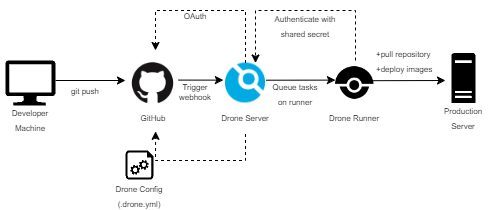
\includegraphics[width=15.0truecm]{images/droneCI.png}
    \caption{Drone (CI/CD)}
    \label{fig:Drone(CI/CD)}
\end{figure}

Miután a Drone Runnerek sikeresen lefuttatták a pipeline lépéseit és létrehozták a szükséges Docker képeket, ezeket a képeket továbbítják a szerverre. Ott pedig lehúzzák és telepítik ezeket a képeket, így az új verziójú alkalmazás azonnal elérhetővé válik az éles környezetben. Ez a folyamat nagyban hozzájárul a szoftverfejlesztés hatékonyságának és a kiadások megbízhatóságának növeléséhez.
\section{Felhaszn\'al\'oi felület}
Ebben a fejezetben részletesen elemzem a felhasználói felületet, ami a szoftver leglátványosabb és közvetlenül érintett része. Bemutatom a felhasználói interakciók kulcsfontosságú pontjait, a navigációs struktúrát és az egyes komponensek funkcionális jelentőségét az alkalmazásban való hatékony mozgás elősegítésére.
\subsection{Bejelentkez\'es}
Itt található a felület, ahol a felhasználók azonosíthatják magukat a rendszerben a regisztráció során megadott adatok felhasználásával. Ezen a ponton van lehetőség a felhasználóknak az új felhasználói fiókok létrehozásának kezdeményezésére is.
\begin{figure}[H]
    \centering
    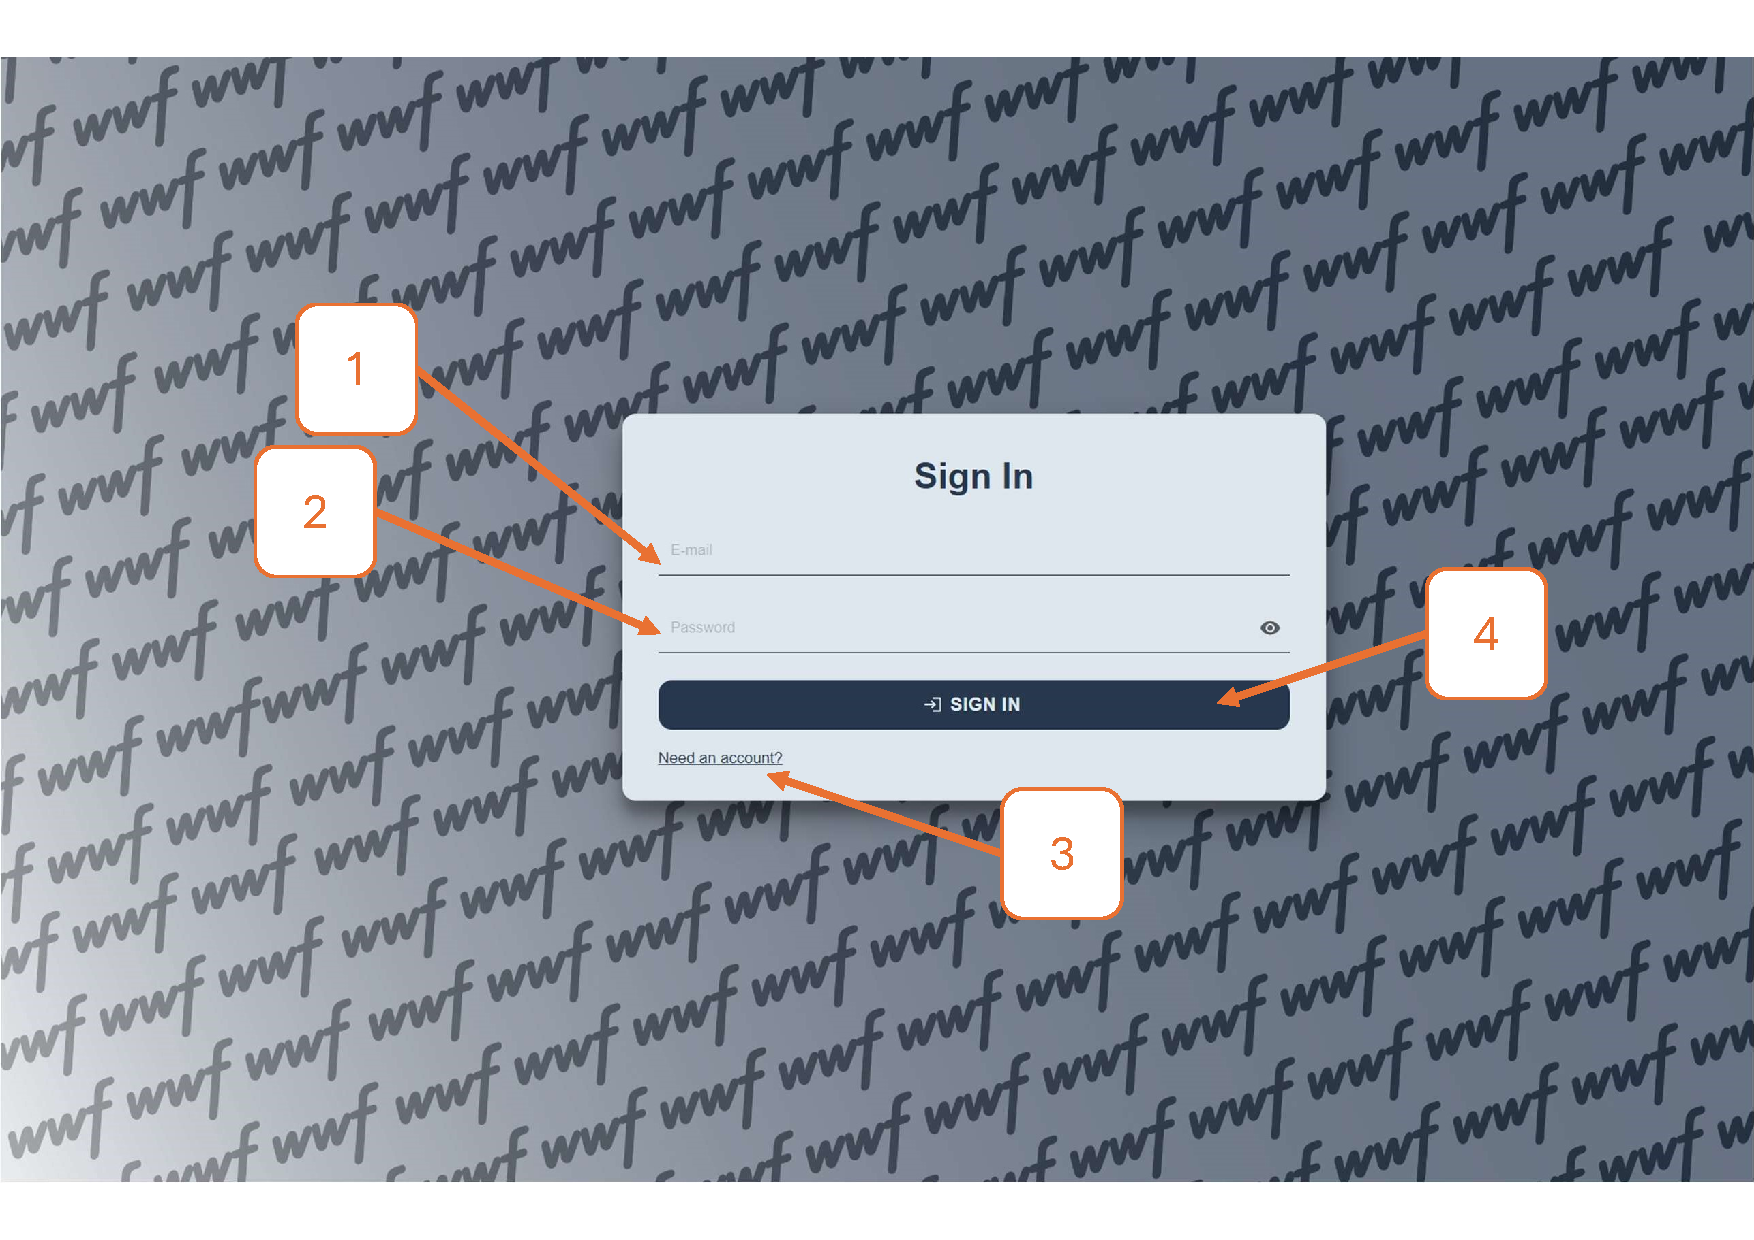
\includegraphics[width=14.0truecm]{images/login.pdf}
    \caption{Bejelentkező felület}
    \label{fig:login}
\end{figure}
\begin{enumerate}
  \item \textbf{E-mail cím}: Itt kell megadni a regisztrációkor használt e-mail címet.
  \item \textbf{Jelszó}: A hozzáférési jogosultság ellenőrzésére szolgáló jelszó.
  \item \textbf{Regisztrációs oldalra navigáló link}: Ez a link a regisztrációs felületre irányítja a felhasználót.
  \item \textbf{Hitelesítő gomb}: A belépési adatok ellenőrzését és a kezdő oldalra történő átirányítást kezdeményezi.
\end{enumerate}
\subsection{Regisztr\'aci\'o}
Ezen a modulon keresztül új felhasználók hozhatják létre fiókjukat, megadva az azonosításhoz szükséges és egyéb személyes adatokat.
\begin{figure}[H]
    \centering
    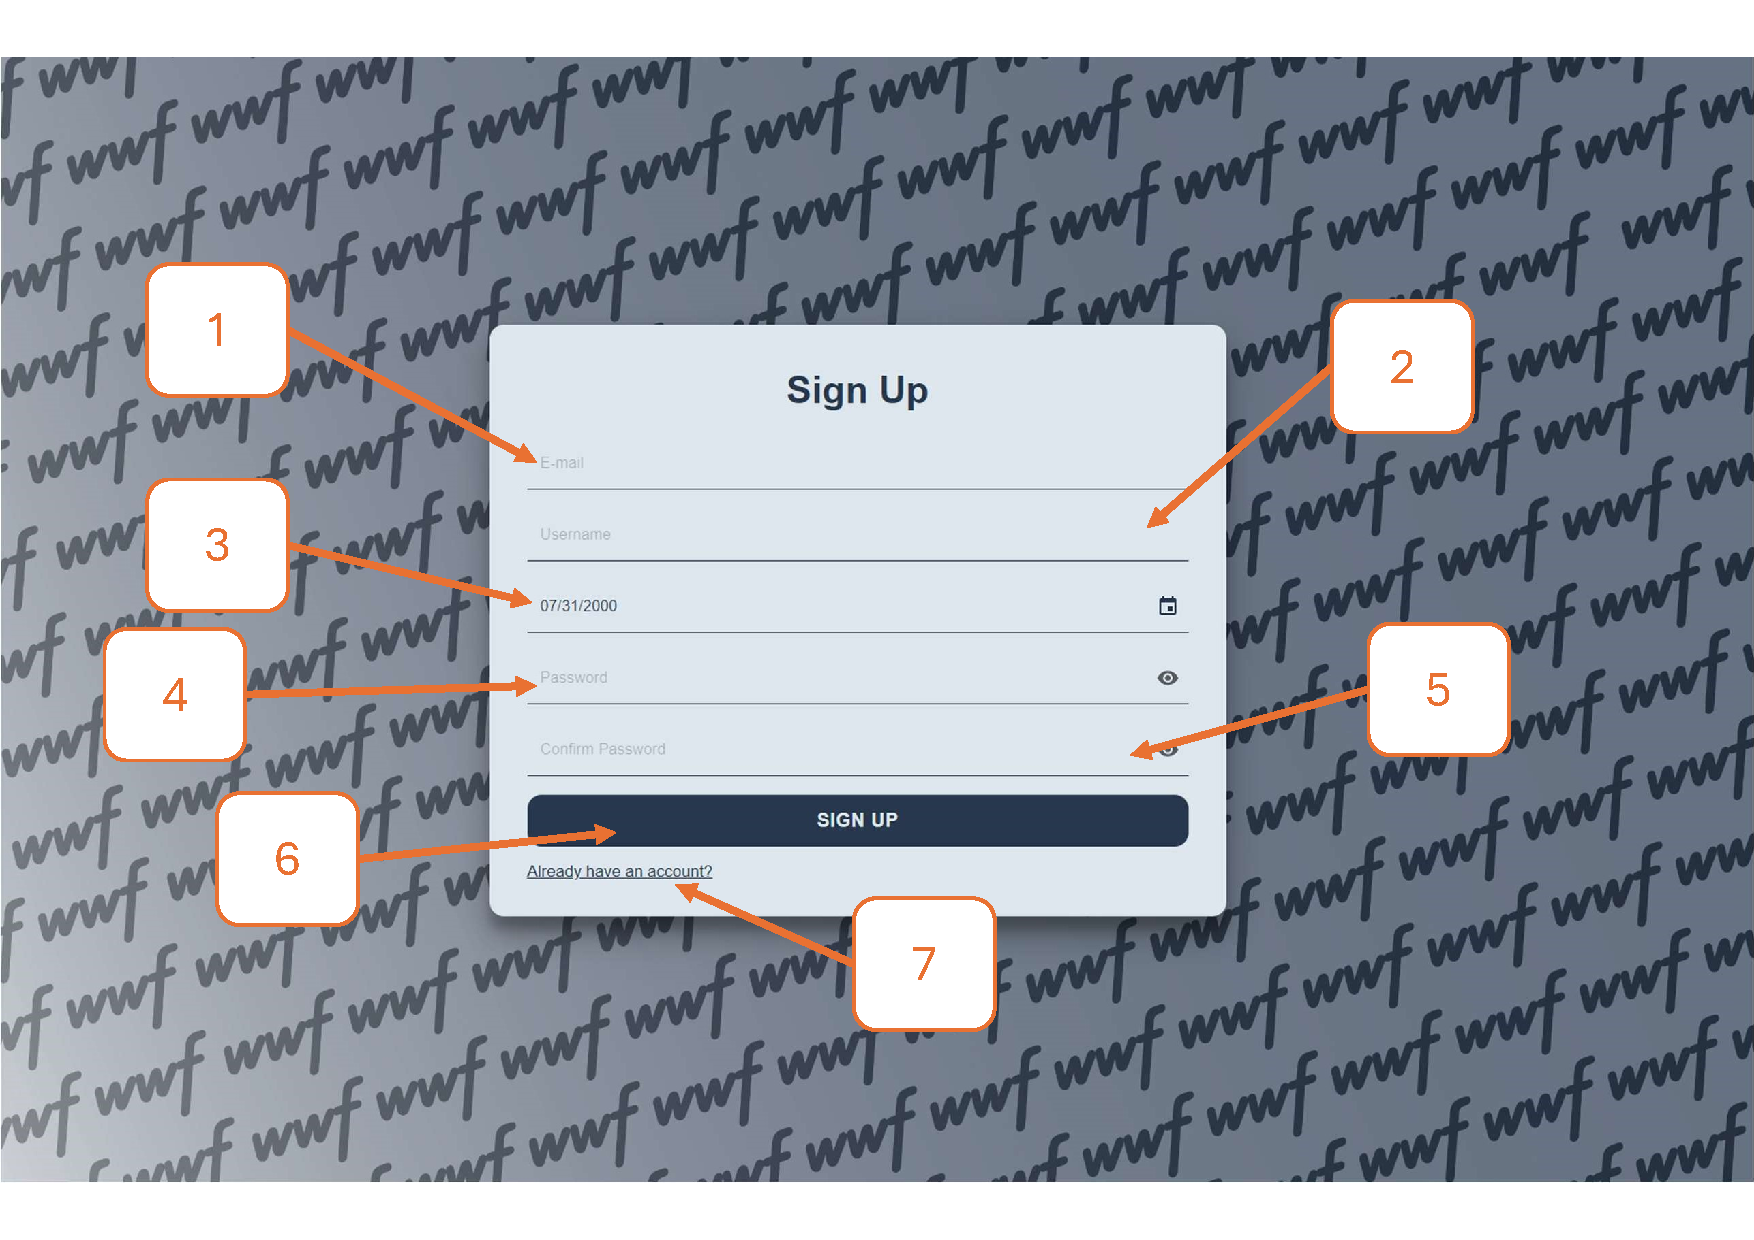
\includegraphics[width=14.0truecm]{images/register.pdf}
    \caption{Regisztrációs felület}
    \label{fig:login}
\end{figure}
\begin{enumerate}
  \item \textbf{Email cím}: A felhasználó által használni kívánt e-mail cím.
  \item \textbf{Felhasználó név}: A felhasználó által választott név, amely más felhasználók számára látható lesz.
  \item \textbf{Születési idő}: A felhasználó életkorának megadása.
  \item \textbf{Jelszó}: Biztonsági kulcsként szolgáló, titkos jelszó.
  \item \textbf{Jelszó megerősítés}: A jelszó helyességének ellenőrzése.
  \item \textbf{Hitelesítő gomb}: A regisztráció véglegesítése és a fiók létrehozása.
  \item \textbf{Bejelentkezési oldalra navigáló link}: A már meglévő felhasználók ezen a linken keresztül navigálhatnak vissza a bejelentkezési felületre.
\end{enumerate}
\begin{figure}[H]
    \centering
    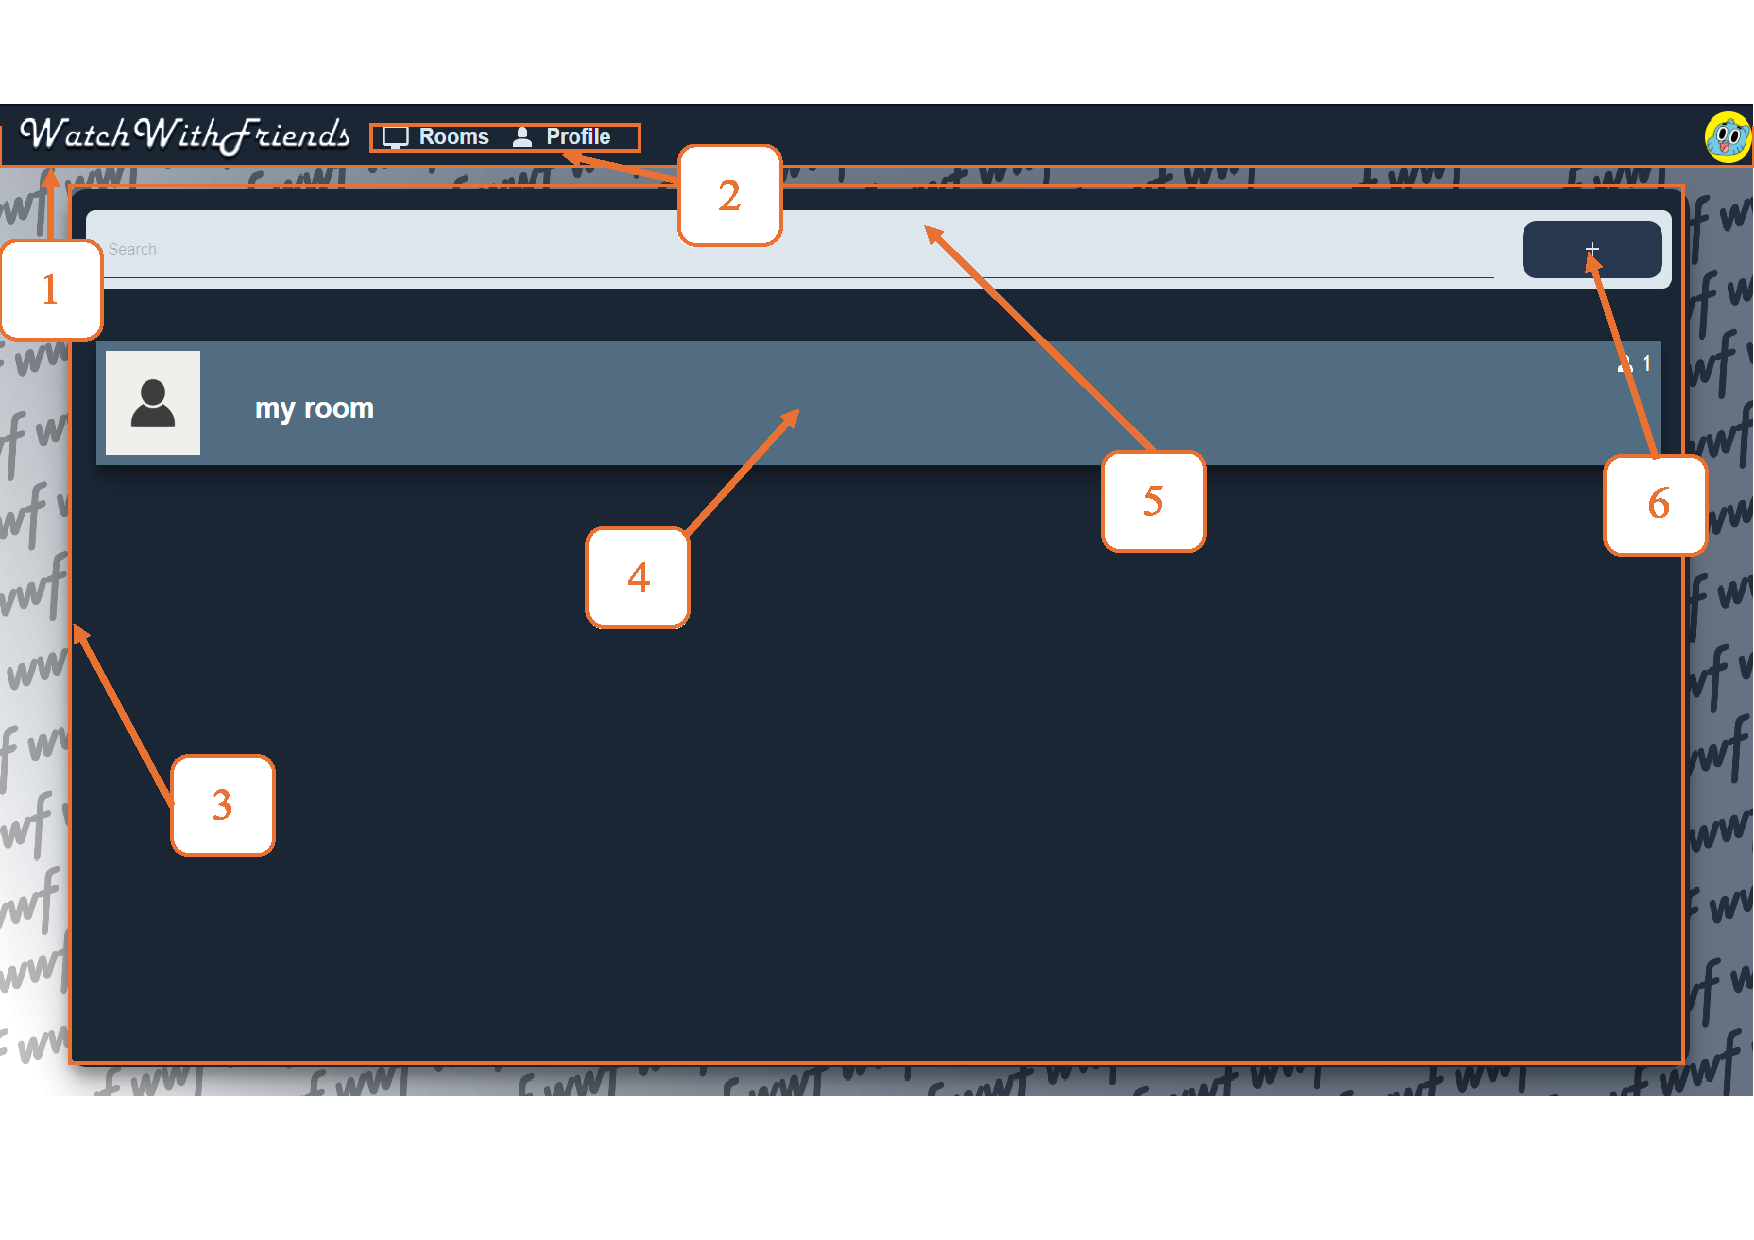
\includegraphics[width=14.0truecm]{images/lobby.pdf}
    \caption{Szobák}
    \label{fig:login}
\end{figure}
\begin{enumerate}
  \item \textbf{Navigációs panel}: Ez a szekció a felhasználó általános navigációs eszközei és az alkalmazás főbb területei közötti átjárhatóságot biztosítja.
\item \textbf{Navigációs linkek}: A felhasználói profil képe és a navigációs linkek gyűjtőhelye.
\item \textbf{Szobák listája}: Szobák keresése, új szoba létrehozása és a meglévő szobák megjelenítése.
\item \textbf{Szoba}: Belépési pont a kiválasztott szobába, szobainformációkkal és aktív tagok számával.
\item \textbf{Kereső mező}: Specifikus szobák gyors megtalálása.
\item \textbf{Szoba létrehozó gomb}: Új szoba létrehozásának kezdeményezése.
\end{enumerate}
\subsection{Profil szerkeszt\'ese}
Ezen a felületen a felhasználók módosíthatják adataikat, beleértve az e-mail címet, felhasználói nevet, profil képet és jelszót.
\begin{figure}[H]
    \centering
    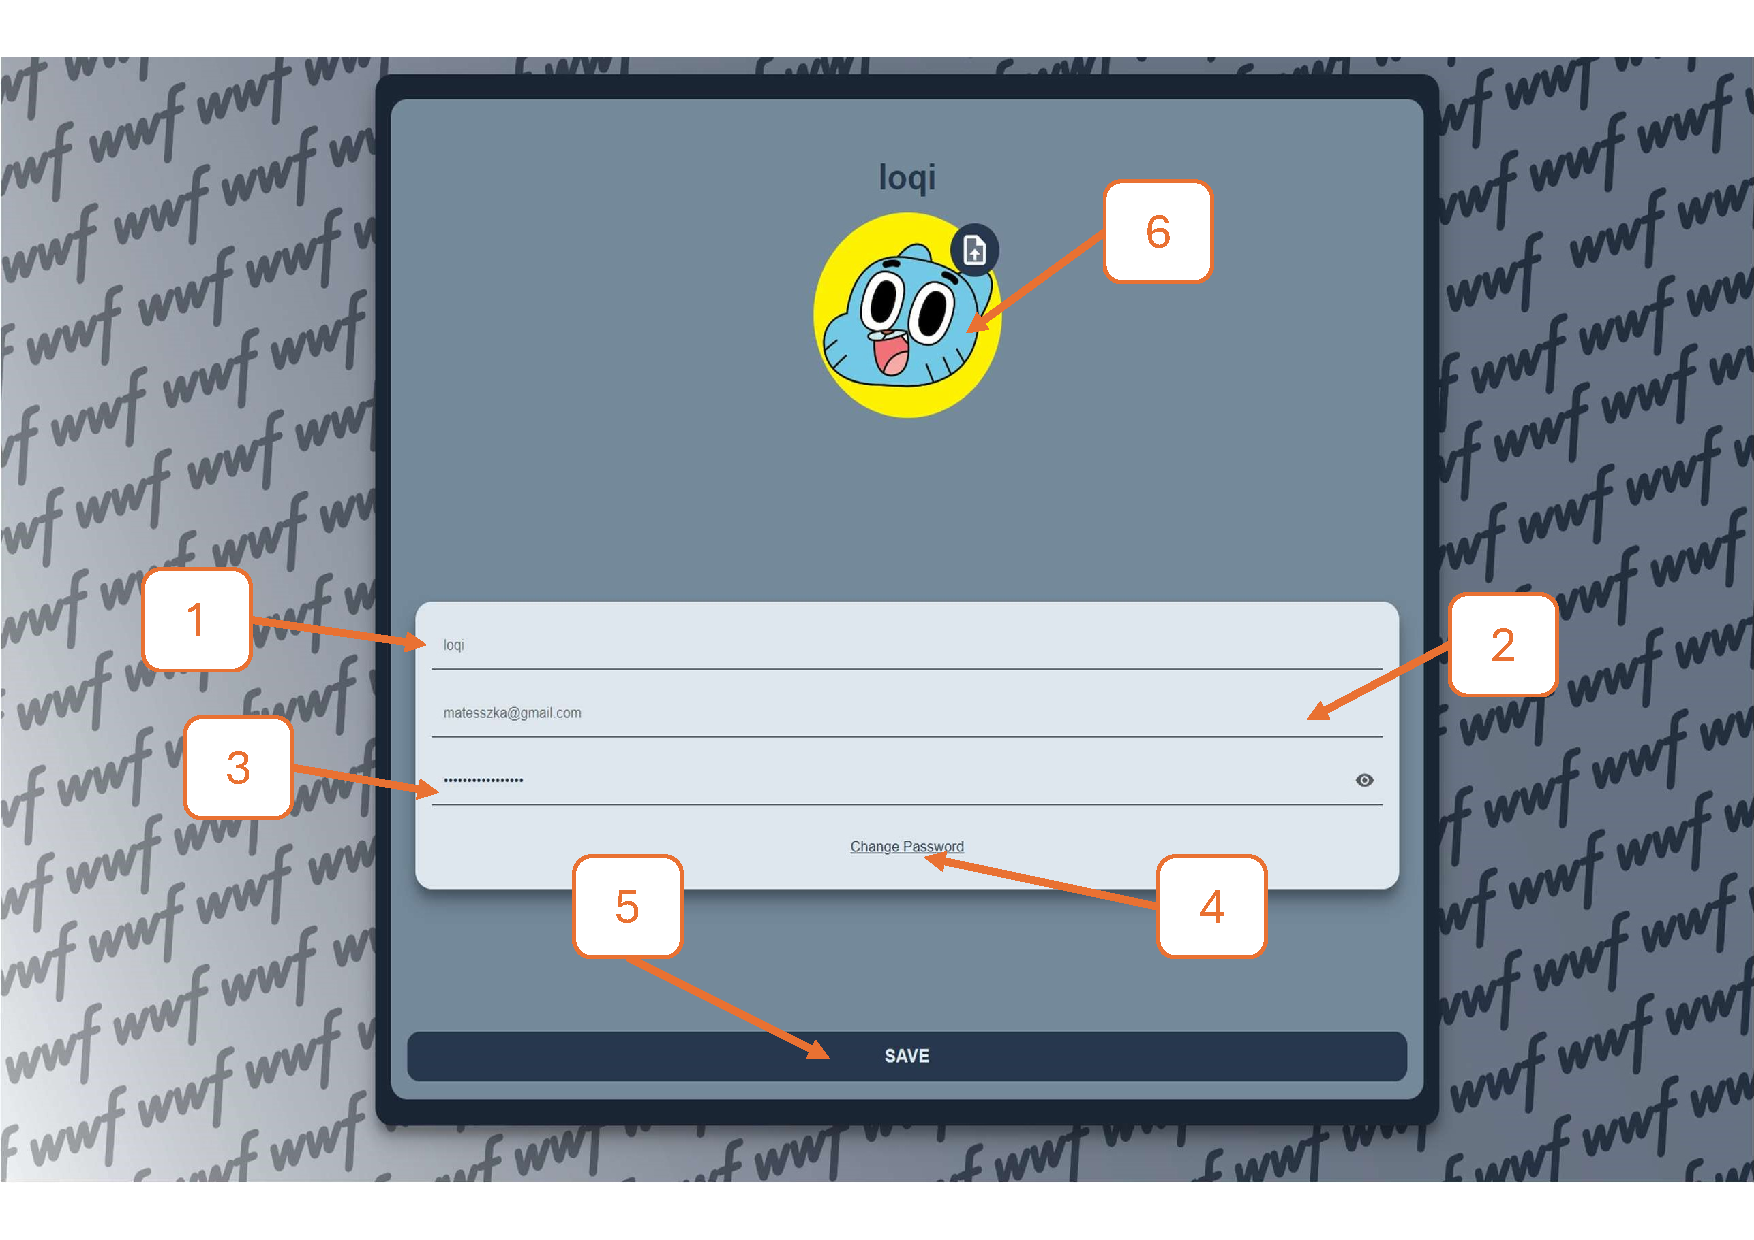
\includegraphics[width=14.0truecm]{images/profil.pdf}
    \caption{Profil szerkesztése}
    \label{fig:login}
\end{figure}
\begin{enumerate}
  \item \textbf{Felhasználó név}: A felhasználó által választott név módosítása.
  \item \textbf{E-mail cím}: Az e-mail cím frissítése.
  \item \textbf{Jelszó}: A hitelesítéshez szükséges jelszó.
  \item \textbf{Jelszó változtatás gomb}: A jelszó megváltoztatásának kezdeményezése.
  \item \textbf{Mentés gomb}: A módosított adatok mentése.
  \item \textbf{Profil kép}: A felhasználói profil képének frissítése.
\end{enumerate}
\subsection{Szoba}
A felhasználók itt tudnak közösen videókat nézni, chat-elni és élményeiket a videóval kapcsolatban, miközben együtt élvezik a tartalmat. Az interaktív chat lehetőséget nyújt arra, hogy a felhasználók egymás reakcióit láthassák és válaszolhassanak rájuk valós időben, ami még személyesebbé és közösségibbé teszi a videózási élményt.
\begin{figure}[H]
    \centering
    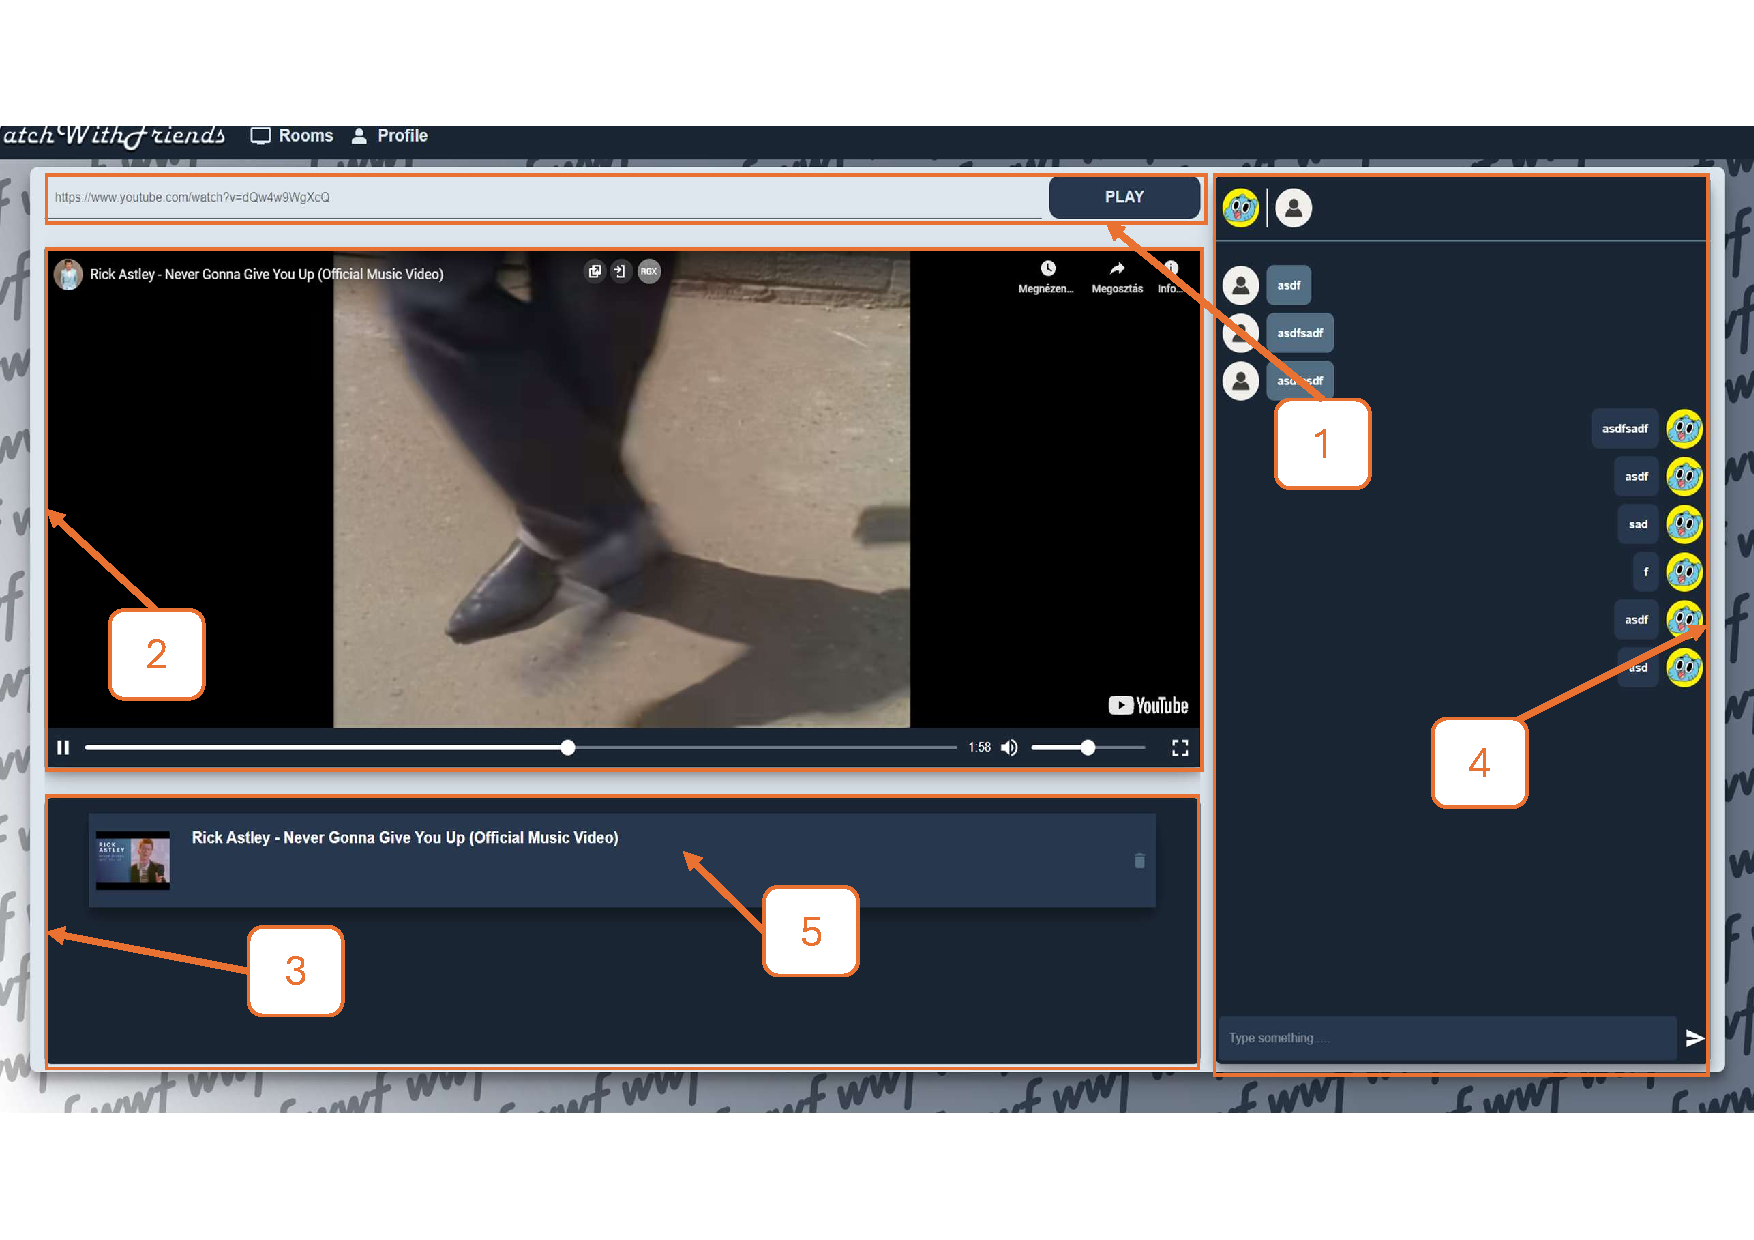
\includegraphics[width=14.0truecm]{images/room.pdf}
    \caption{Szoba felülete}
    \label{fig:login}
\end{figure}
\begin{enumerate}[label=\textbf{\arabic*.}]
    \item \textbf{Videó Hozzáadási Felület}: Ez az eszköz lehetővé teszi a felhasználók számára, hogy közvetlen URL-címek megadásával új videókat adjanak hozzá a megosztásra szánt listához. A felhasználók így egyszerűen megoszthatnak tartalmakat a többi résztvevővel.
    
    \item \textbf{Videó Lejátszó}: A képernyő középső részén található, a kiválasztott videó megjelenítésére szolgáló rész. Itt lehetőség van a videó lejátszásának kezdésére, szüneteltetésére, és más, a lejátszással kapcsolatos beállítások elvégzésére.
    
    \item \textbf{Lejátszási Lista}: Egy panel ahol a megosztásra váró vagy már megosztott videók listája látható. 
    
    \item \textbf{Chat}: A jobb oldali chat panelen keresztül a felhasználók írhatnak egymásnak üzeneteket, kommentálhatják a videókat, vagy egymással diskurálhatnak valós időben. Ez a közösségi interakció fontos része a közös videózás élményének.
    
    \item \textbf{Lejátszási Lista Elem}: Egy konkrét videó, amit a lejátszási listára helyeztek, tartalmazza a videó címét és előnézeti képét. 
\end{enumerate}


Ezek a felületek és funkciók együttesen szolgálják a felhasználók zökkenőmentes és hatékony interakcióját az alkalmazáson belül, elősegítve a felhasználói élmény javítását és az alkalmazás hatékony használatát.